\documentclass[ngerman,12pt]{scrartcl}

\usepackage[utf8]{inputenc}
\usepackage[T1]{fontenc}
\usepackage{babel}

\usepackage{palatino}
\usepackage{microtype}
\usepackage{paralist}
\usepackage{blindtext}

\usepackage{graphicx} % nicht graphics
% JPG, PNG, PDF

\usepackage{hyperref}
\hypersetup{
    bookmarks=true,                     % show bookmarks bar
    unicode=false,                      % non - Latin characters in Acrobat’s bookmarks
    pdftoolbar=true,                        % show Acrobat’s toolbar
    pdfmenubar=true,                        % show Acrobat’s menu
    pdffitwindow=false,                 % window fit to page when opened
    pdfstartview={FitH},                    % fits the width of the page to the window
    pdftitle={My title},                        % title
    pdfauthor={Author},                 % author
    pdfsubject={Subject},                   % subject of the document
    pdfcreator={Creator},                   % creator of the document
    pdfproducer={Producer},             % producer of the document
    pdfkeywords={keyword1, key2, key3},   % list of keywords
    pdfnewwindow=true,                  % links in new window
    colorlinks=true,                        % false: boxed links; true: colored links
    linkcolor=blue,                          % color of internal links
    filecolor=cyan,                     % color of file links
    citecolor=green,                     % color of file links
    urlcolor=magenta                        % color of external links
}



\title{Mein erstes \LaTeX-Dokument}
\author{Uwe Ziegenhagen}
\date{Köln, den 11.06.2021}


\begin{document}
\maketitle

\tableofcontents

\listoffigures

\section{Einleitung}

Hallo Fernuni Hagen! Siehe Abschnitt \ref{sec:anhang} oder Abbildung \ref{fig:melli} auf Seite \pageref{fig:melli}.

\section{Hauptteil}
\subsection{Literaturüberblick}

\begin{itemize}
\item Hallo
\item Ich 
\item bin 

\begin{itemize}
\item Hallo
\item Ich 
\item bin 
\item eine Liste mit Bulletpunkten
\end{itemize}

\item eine Liste mit Bulletpunkten
\end{itemize}

\begin{compactitem}[?]
\item Hallo
\item Ich 
\item bin 
\item eine Liste mit Bulletpunkten
\end{compactitem}

\begin{enumerate}[I] % große römische Zeichen
\item Hallo
\item Ich 
\item bin 
\item eine nummerierte Liste
\end{enumerate}

\begin{compactenum}
\item Hallo
\item Ich 
\item bin 
\item eine nummerierte Liste
\end{compactenum}

\begin{description}
\item [Mehl] 1 Tasse
\item [Milch] 500 Milliliter
\item [Backpulver und weitere Zutaten] 1 Packung
\end{description}


\begin{compactdesc}
\item [Mehl] 1 Tasse
\item [Milch] 500 Milliliter
\item [Backpulver und weitere Zutaten] 1 Packung
\end{compactdesc}

\subsubsection{Moderne Literatur}

\blindtext[100]

\section{Zusammenfassung}

In diesem Artikel konnten wir beweisen, dass

\paragraph{Altertum} \blindtext

\paragraph{Neuzeit} \blindtext

\section{Anhang}\label{sec:anhang}


Die Materialien können frei von jedermann genutzt und verändert werden, entsprechende Hinweise auf meine Urheberschaft werden aber gern gesehen.

Die Materialien können frei von jedermann genutzt und verändert werden, entsprechende Hinweise auf meine Urheberschaft werden aber gern gesehen.

Ein Editor zur Bearbeitung der TeX-Dateien: TeX Live bringt für Mac und Windows TeXworks mit, einen guten Editor, den ich gern benutze. 
TeX Studio und Visual Studio Code (mit der LaTeX Workshop Erweiterung von James Yu) kann ich ebenfalls sehr empfehlen.


\includegraphics[width=5cm]{Bilder/miau}


\includegraphics[width=0.5\textwidth]{Bilder/miau} % halbe Textbreite


\includegraphics[width=\textwidth,angle=45]{Bilder/miau} % Textbreite

\blindtext[3]

\begin{figure}[b] % h = here, t = top, b = bottom
\centering

\includegraphics[width=0.75\textwidth]{Bilder/miau} % Textbreite
\caption{Ich bin Melli}\label{fig:melli}
\end{figure}

\begin{figure}[t] % h = here, t = top, b = bottom
\centering

\includegraphics[width=0.75\textwidth]{Bilder/melli} % Textbreite
\caption{Ich bin Melli}\label{fig:melli2}
\end{figure}

\blindtext[3]

\begin{figure}[t] % h = here, t = top, b = bottom
\centering
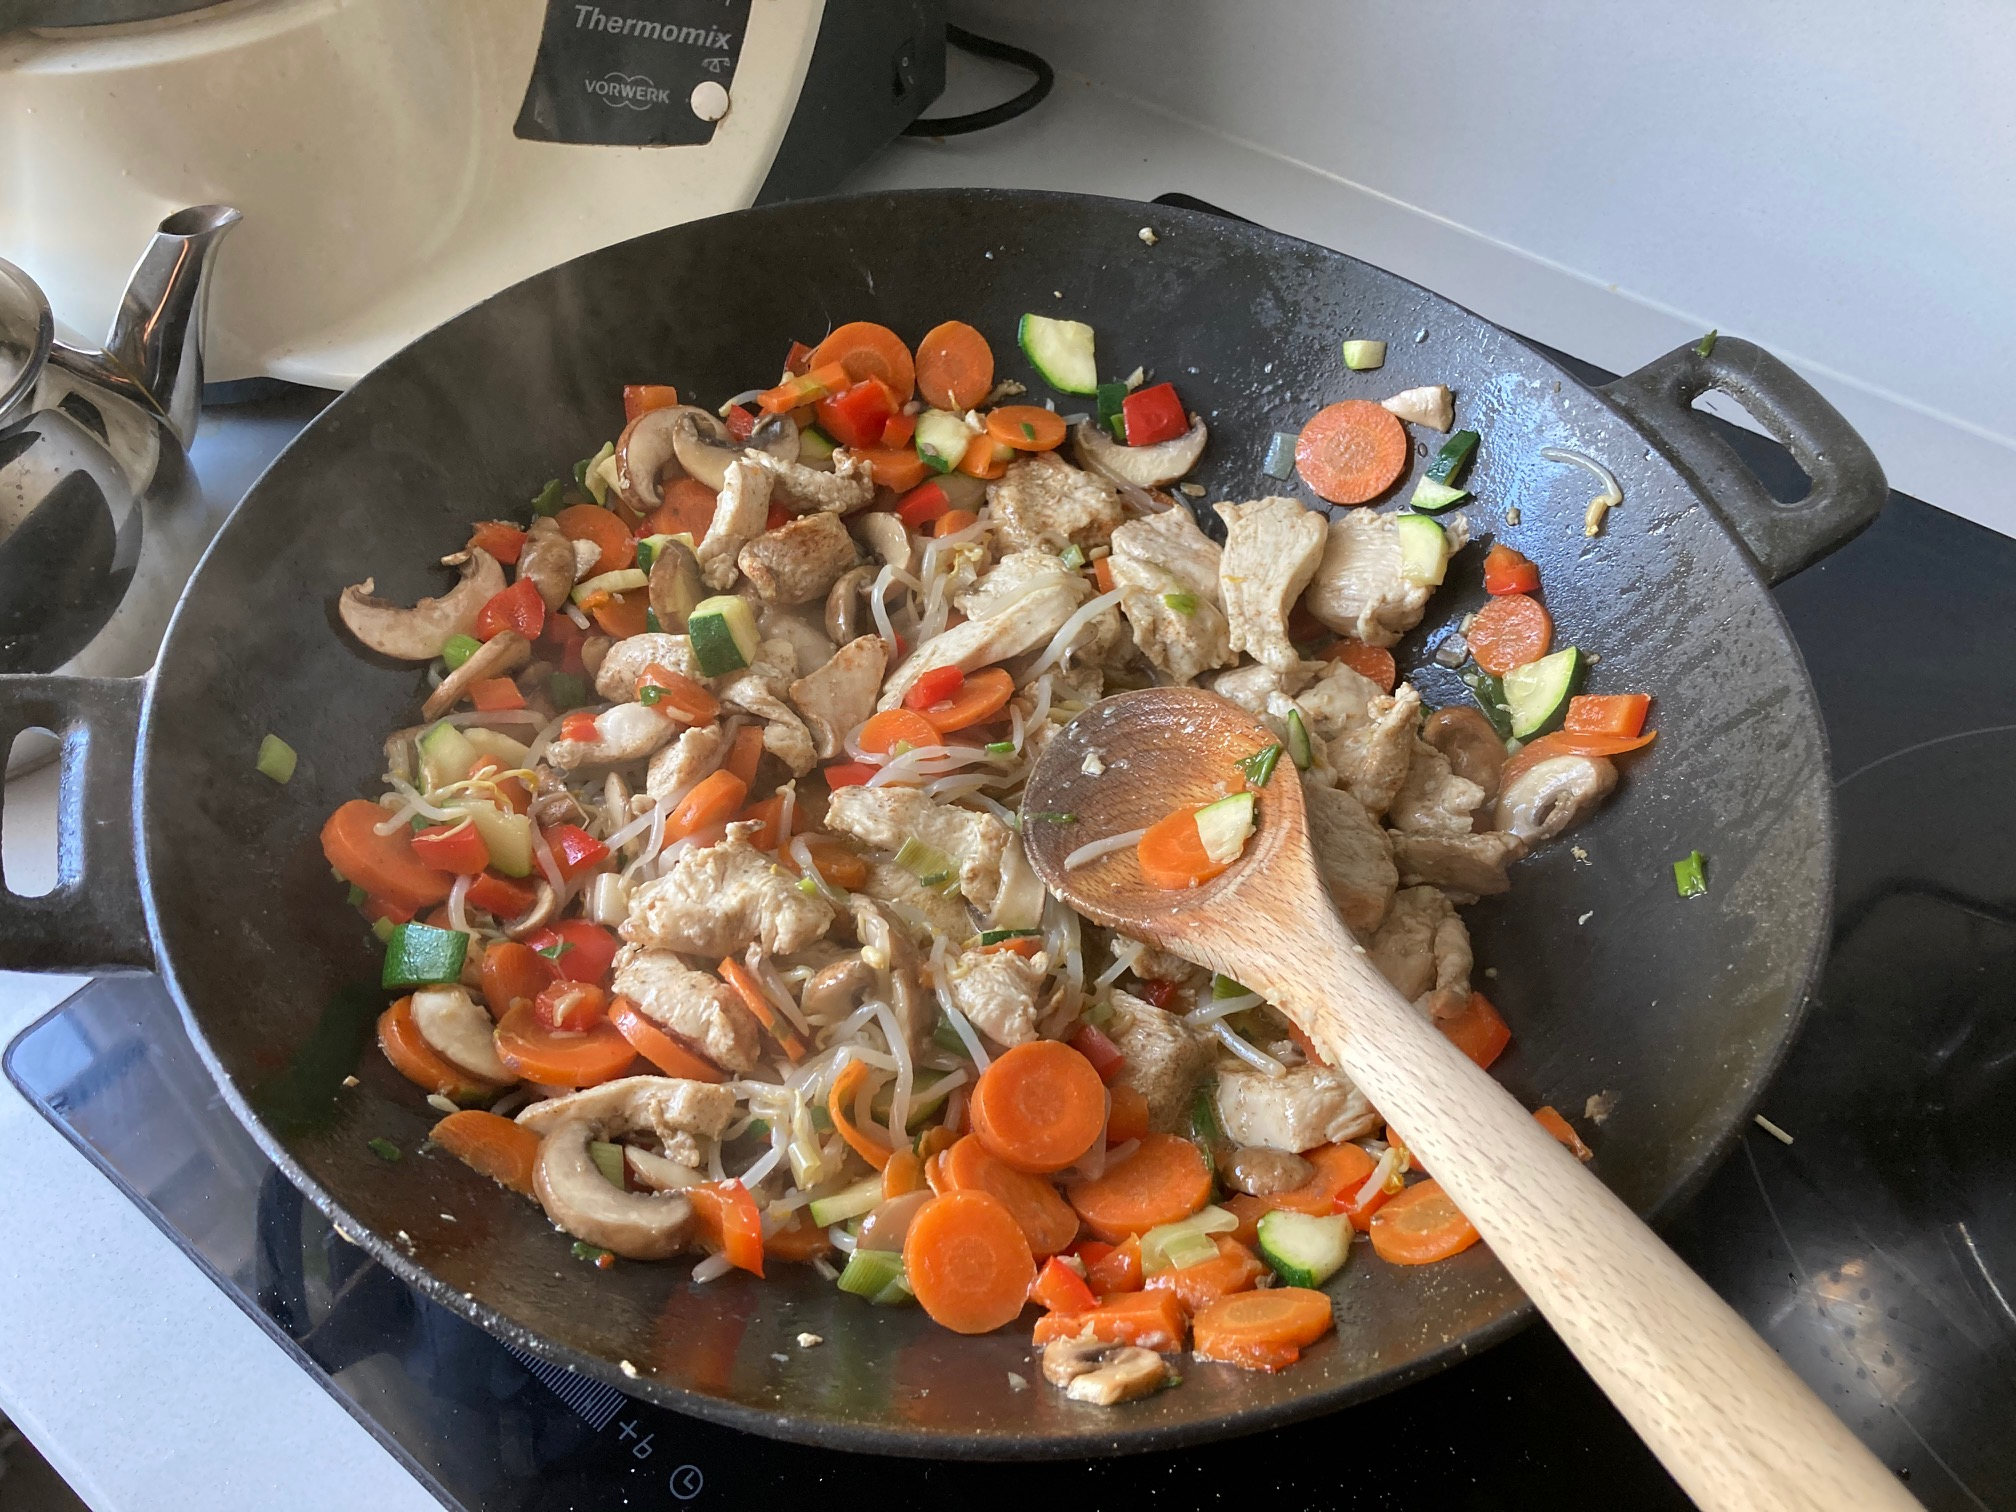
\includegraphics[width=0.75\textwidth]{Bilder/essen1} % Textbreite
\caption{Selbstgekochtes}\label{fig:essen1}
\end{figure}

\begin{figure}[t] % h = here, t = top, b = bottom
\centering
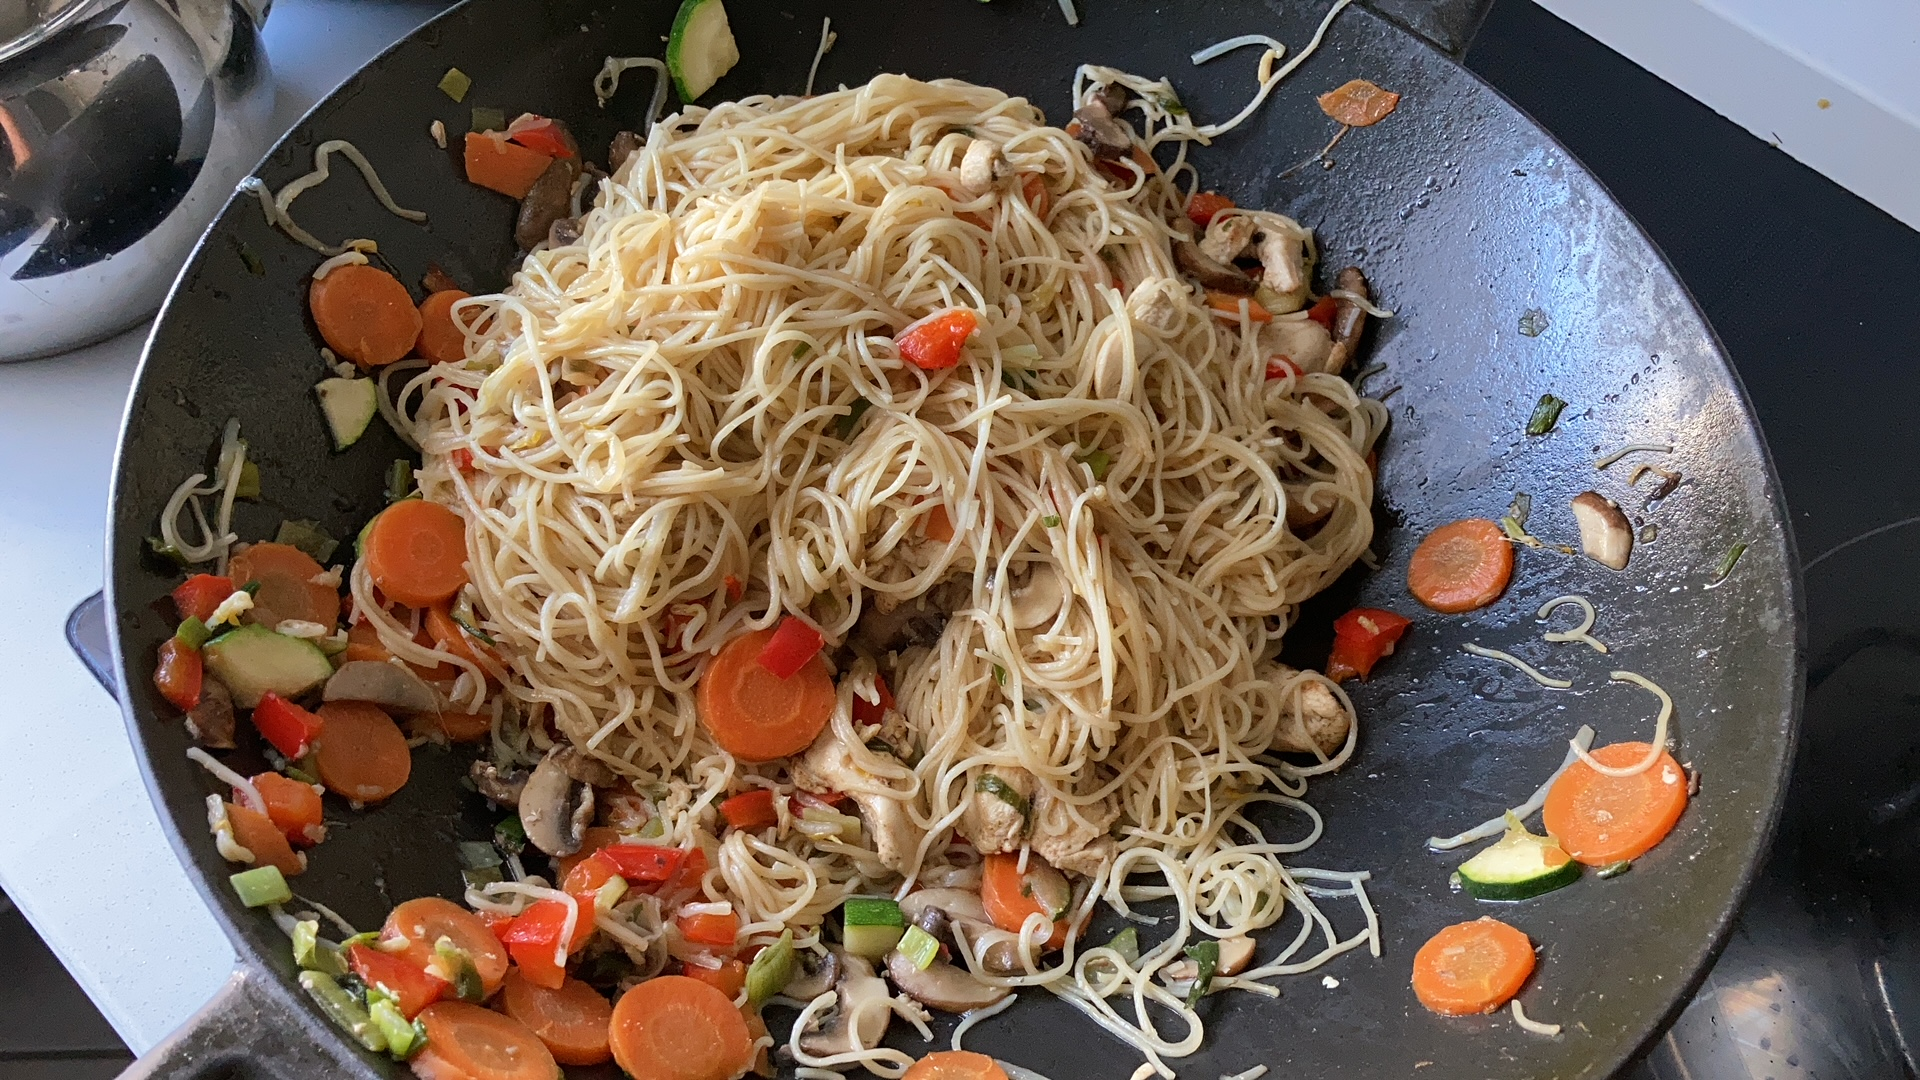
\includegraphics[width=0.75\textwidth]{Bilder/essen2} % Textbreite
\caption{Selbstgekochtes Nummer 2}\label{fig:essen2}
\end{figure}


\blindtext[3]


\begin{figure}[b] % h = here, t = top, b = bottom

\includegraphics[width=0.5\textwidth]{Bilder/miau} % Textbreite
\caption{Ich bin Melli}\label{fig:melli}
\end{figure}

\begin{figure}[b] % h = here, t = top, b = bottom
\hfill

\includegraphics[width=0.5\textwidth]{Bilder/miau} % Textbreite
\caption{Ich bin Melli}\label{fig:melli}
\end{figure}


\end{document}




